La programmazione concorrente, programma visto come composizione di numerose attività autonome, è l'elemento più importante di questi tempi.
I server web gestiscono richieste per migliaia di client contemporaneamente.
Le app degli smartphone e dei tablet gestiscono le animazioni sull'interfaccia utente mentre simultaneamente eseguono la computazione e le richieste di rete in background.
Anche i tradizionali problemi di batch (lettura dei dati, computazione e scrittura degli output) usano la concorrenza per nascondere la latenza delle operazioni I/O così da sfruttare anche i multiprocessori dei computer moderni, i quali, negli anni, continuano a crescere in numero ma non in velocità.

Go offre due stili di programmazione concorrente.
In questo capitolo vengono esponte le goroutine e i channel, compatibili con la \textit{CSP} o \textit{communicating sequential processes}, un modello di concorrenza dove i valori sono visti come attività indipendenti (goroutine), ma con le variabili confinate alle singole attività.
Nel prossimo capitolo verranno illustrati gli aspetti più tradizionali del modello \textit{shared memory multithreading}.


\section{Goroutine}
\label{sec:goroutine}%
In Go, ogni attività concorrente in esecuzione è detta \textit{goroutine}.
Dato un programma con due funzioni, uno che svolge operazioni di computazione e l'altra che scrive qualche dato in output, si supponga che entrambi non si richiamino a vicenda.
Un programma sequenziale potrebbe chiamare una funzione e solo in seguito l'altra, ma in un programma \textit{concorrente} con due o più goroutine, le chiamate ad \textit{entrambe} le funzioni possono essere svolte contemporaneamente.

Si può pensare per ora alle goroutine come a thread perché la loro differenza è essenzialmente in termini quantitativi e non qualitativi.

Quando un programma viene avviato, la sua unica goroutine è quella che richiama la funzione \verb|main|, definita \textit{main goroutine}.
Le nuove goroutine sono create dall'istruzione \verb|go|.
Sintatticamente, un'istruzione \verb|go| è una funzione ordinaria o una chiamata ad un metodo con la parola chiave \verb|go| come prefisso.
Un'istruzione \verb|go| permette alla funzione di essere chiamata da una nuova e goroutine.
\begin{lstlisting}[frame=single, label={lst:lstlisting7-1.1}]
f()    // chiama f(); attende il risultato
go f() // crea una nuova goroutine che chiama f(); non c'%*\textit{è}*\)
       // attesa
\end{lstlisting}
Nel seguente esempio, la main goroutine computa il 45esimo numero di Fibonacci.
Dato che utilizza un algoritmo inefficiente, essa rimarrà in esecuzione per un tempo considerevole, durante il quale si vorrebbe dire all'utente che il programma è ancora in esecuzione tramite la stampa di uno ``spinner'' testuale.
\begin{lstlisting}[frame=single, label={lst:lstlisting7-1.2}]
func main() {
    go spinner(100 * time.Millisecond)
    const n = 45
    fibN := fib(n) // lento
    fmt.Printf(%*``*\)\rFibonacci(%d) = %d\n%*''*\), n, fibN)
}

func spinner(delay time.Duration) {
    for {
        for _, r := range `-\|/' {
            fmt.Printf(%*``*\)\r%c%*''*\), r)
            time.Sleep(delay)
        }
    }
}
\end{lstlisting}
\begin{lstlisting}[frame=single, label={lst:lstlisting7-1.3}]
func fib(x int) int {
    if x < 2 {
        return x
    }
    return fib(x-1) + fib(x-2)
}
\end{lstlisting}
Una volta computato il risultato, la funzione \verb|main| lo stampa e quindi effettua il return.
Quando questo succede, tutte le goroutine vengono bruscamente terminate e il programma si chiude.
Non esistono altri modi per terminare una goroutine se non chiudere il programma o effettuare il return della funzione \verb|main|, questo perché una goroutine non può terminarne un'altra;
esistono tuttavia possibilità di metterle in comunicazione.


\section{Esempio: clock server concorrente}
\label{sec:esempio_clock_server_concorrente}
%
La rete è un dominio naturale dove usare la concorrenza perché vengono tipicamente gestite molte connessioni provenienti da diversi client allo stesso tempo, consci che ogni client è in genere indipendente da tutti gli altri.

Esponiamo come primo esempio un clock server sequenziale che scrive l'orario corrente al client ad ogni secondo:
\begin{lstlisting}[frame=single, label={lst:lstlisting7-2.1}]
// Clock1 %*\textit{è}*\) un server TCP che periodicamente scrive l'orario.
func main() {
    listener, err := net.Listen(%*``*\)tcp%*''*\), %*``*\)localhost:8000%*''*\))
    if err != nil {
        log.Fatal(err)
    }
    for {
        conn, err := listener.Accept()
        if err != nil {
            log.Print(err) // p.e., connessione fallita
            continue
        }
        handleConn(conn) // gestisce una connessione alla volta
    }
}

func handleConn(c net.Conn) {
    defer c.Close()
    for {
        _, err := io.WriteString(c,
            time.Now().Format(%*``*\)15:04:05\n%*''*\)))
        if err != nil {
            return // p.e., client disconnesso
        }
        time.Sleep(1 * time.Second)
    }
}
\end{lstlisting}
La funzione \verb|Listen| crea un \verb|net.Listener|, un oggetto che ``ascolta'' l'arrivo di connessioni in ingresso sullo porta di rete designata, in questo caso la porta TCP \verb|localhost:8000|.
Il metodo \verb|Accept| del listener blocca il listener stesso in attesa di una richiesta di connessione, quindi restituisce un oggetto \verb|net.Conn| rappresentante la connessione attesa.

La funzione \verb|handleConn| gestisce una completa connessione del client.
In un ciclo, essa scrive l'orario corrente, \verb|time.Now()|, al client.
Finché \verb|net.Conn| soddisfa l'interfaccia \verb|io.Writer|, si può scrivere direttamente al client.
Il ciclo finisce quando la scrittura fallisce, che molto probabilmente accade quando il client si disconnette, momento in cui \verb|handleConn| chiude il proprio lato della connessione usando la chiama differita a \verb|Close| e torna ad attendere la richiesta di una connessione.

Sul lato client il programma è il seguente:
\begin{lstlisting}[frame=single, label={lst:lstlisting7-2.2}]
// Netcat1 %*\textit{è}*\) un client TCP di sola lettura
func main() {
    conn, err := net.Dial(%*``*\)tcp%*''*\), %*``*\)localhost:8000%*''*\))
    if err != nil {
        log.Fatal(err)
    }
    defer conn.Close()
    mustCopy(os.Stdout, conn)
}

func mustCopy(dst io.Writer, src io.Reader) {
    if _, err := io.Copy(dst, src); err != nil {
        log.Fatal(err)
    }
}
\end{lstlisting}
Questo programma legge i dati dalla connessione e li scrive sullo standard output fino a quando non viene incontrato una condizione di end-of-file o un errore.
Eseguendo due client allo stesso tempo si esegue il seguente risultato:
\begin{lstlisting}[language=bash, frame=L, label={lst:lstlisting7-2.3}]
$ ./netcat1
13:56:34
13:56:35        $ ./netcat1
13:56:36
^C
                13:56:38
                13:56:39
                13:56:40
                ^C
\end{lstlisting}
In questa implementazione il secondo client è obbligato ad aspettare che il primo client finisca perché il server è \textit{sequenziale};
il server si occupa di un client alla volta.
Per rendere il server concorrente serve solo una piccola modifica: l'aggiunta della parola chiave \verb|go| alla chiamata di \verb|handleConn| fa sì che ogni chiamata venga eseguita nella propria goroutine.
\begin{lstlisting}[frame=single, label={lst:lstlisting7-2.4}]
func main() {
    listener, err := net.Listen(%*``*\)tcp%*''*\), %*``*\)localhost:8000%*''*\))
    if err != nil {
        log.Fatal(err)
    }
    for {
        conn, err := listener.Accept()
        if err != nil {
            log.Print(err) // p.e., connessione fallita
            continue
        }
        go handleConn(conn) // gestisce le connessioni in modo
                            // concorrente
    }
}
\end{lstlisting}
Ora più client possono ricevere l'orario contemporaneamente:
\begin{lstlisting}[language=bash, frame=L, label={lst:lstlisting7-2.5}]
$ ./netcat2
13:58:54
13:58:55        $ ./netcat2
13:58:56        13:58:56
13:58:57        13:58:57
13:58:58        13:58:58
13:58:59        ^C
13:59:00
13:59:01        $ ./netcat2
13:59:02        13:59:02
13:59:03        13:59:03
^C              13:59:04
                ^C
\end{lstlisting}

\section{I channel}
\label{sec:channel}
%
Se in Go le goroutine sono le attività di un programma concorrente, i channel sono le connessioni fra di loro.
Un channel è un meccanismo di comunicazione che permette di inviare valori ad un'altra goroutine.
Ogni channel è un condotto per i valori di un tipo particolare, detto \textit{tipo elementare} del channel.
Il tipo del channel che ha elementi di tipo \verb|int| è indicato come \verb|chan int|.

Per creare un channel viene usata la funzione built-in \verb|make|:
\begin{lstlisting}[frame=single, label={lst:lstlisting7-4.1}]
ch := make(chan int) // ch ha tipo `chan int'
\end{lstlisting}
Come per le map, un channel è un \textit{riferimento} ad una struttura dati creata da \verb|make|.
Quando si fa una copia ad un channel o quando viene passato come argomento ad una funzione, in realtà se ne sta copiando il riferimento, così il chiamante e il chiamato si riferiranno alla stessa struttura dati.
Come per gli altri tipi referenziati, il valore zero di un channel è il \verb|nil|.

Due channel dello stesso tipo possono essere confrontati con \verb|==|.
Il confronto è vero se entrambi sono riferimenti alla stessa struttura dati channel.
Un channel può anche essere confrontato con un \verb|nil|.

Un channel ha due operazioni principali, \textit{send} e \textit{receive}, conosciuti insieme come operazioni di \textit{communication}.
Un operazione di send trasmette, per mezzo del channel, un valore da una goroutine ad un altra goroutine che esegue una corrispondente operazione di receive.
Entrambe le operazioni sono scritte usando l'operatore \verb|<-|.
In un'operazione di send, \verb|<-| separa il channel dall'operando valore.
In un'operazione di receive \verb|<-| precede l'operando channel.
Un'operazione di receive il cui risultato non viene utilizzato è un'istruzione valida.
\begin{lstlisting}[frame=single, label={lst:lstlisting7-4.2}]
ch <- x // un'istruzione di send

x = <-ch // un'espressione di receive in un'operazione di
         // assegnamento
<-ch     // un'istruzione di receive; il risultato %*\textit{è}*\) scartato
\end{lstlisting}
I channel supportano una terza operazione, \textit{close}, che imposta un flag sul channel ad indicare che nessun valore verrà più inviato tramite esso;
tentare comunque un invio causa un panic.
Le operazioni di receive su un channel chiuso restituiscono i valori che sono stati inviati prima della chiusura fino a quando non finiscono;
qualunque successiva operazione di receive viene risolta immediatamente producendo il valore zero del tipo elementare del channel.

Per chiudere un channel, bisogna chiamare la funzione built-in \verb|close|:
\begin{lstlisting}[frame=single, label={lst:lstlisting7-4.3}]
close(ch)
\end{lstlisting}
Un channel creato con una chiamata a \verb|make| viene detto un \textit{unbuffered} channel, ma \verb|make| accetta un secondo argomento opzionale, un intero detto \textit{capacity} del channel.
Se la capacity del channel è diversa da zero, \verb|make| crea un \textit{buffered} channel.
\begin{lstlisting}[frame=single, label={lst:lstlisting7-4.4}]
ch = make(chan int)    // unbuffered channel
ch = make(chan int, 0) // unbuffered channel
ch = make(chan int, 3) // buffered channel con capacity 3
\end{lstlisting}

\subsection{Unbuffered channel}
\label{subsec:unbuffered_channel}%
Un'operazione di send su un unbuffered channel blocca la goroutine mittente fino a quando un'altra goroutine esegue una corrispondente operazione di receive sullo stesso channel, momento in cui il valore è trasmesso e entrambe le goroutine possono proseguire la loro esecuzione.
Al contrario, se l'operazione di receive viene eseguita prima, la goroutine destinataria viene bloccata fino a quando un'altra goroutine eseguirà una send sullo stesso channel.

La comunicazione su un unbuffered channel costringe le goroutine, mittente e destinatario, a \textit{sincronizzarsi}.
Per questa ragione, gli unbuffered channel sono qualche volta detti channel \textit{sincronizzati}.
Quando un valore è inviato su un unbuffered channel, la ricezione del valore \textit{avviene prima} del risveglio della goroutine mittente.

Quando \textit{x} non viene eseguito nè prima di \textit{y} nè dopo \textit{y}, si dice che \textit{x è concorrente ad y}.
Questo non vuol dire necessariamente che \textit{x} e \textit{y} sono simultanei, piuttosto che non è possibile fare ipotesi sul loro ordine d'esecuzione.

Per far sì che la main goroutine attenda la fine della goroutine in background prima di chiudere il programma, si può usare un channel per sincronizzare le due goroutine:
\begin{lstlisting}[frame=single, label={lst:lstlisting7-4-1.1}]
func main() {
   conn, err := net.Dial(%*``*\)tcp%*''*\), %*``*\)localhost:8000%*''*\))
   if err != nil {
      log.Fatal(err)
   }
   done := make(chan struct{})
   go func() {
      io.Copy(os.Stdout, conn) // NOTA: gli errori sono ignorati
      log.Println(%*``*\)done%*''*\))
      done <- struct{}{} // si avvisa la main goroutine
   }()
   mustCopy(conn, os.Stdin)
   conn.Close()
   <-done // attende la fine della goroutine in background
}

func mustCopy(dst io.Writer, src io.Reader) {
   if _, err := io.Copy(dst, src); err != nil {
      log.Fatal(err)
   }
}
\end{lstlisting}
Quando l'utente chiude lo stream di standard input, \verb|mustCopy| si conclude e la main goroutine chiama \verb|conn.Close()|, chiudendo entrambe le parti della connesione alla rete.
La chiusura del lato scrittura della connessione permette al server di vedere una condizione di end-of-file.
La chiusura del lato lettura della connessione causa alla chiamata di \verb|io.Copy| sulla goroutine in background di restituire un errore ``read from closed connection'' (lettura da una connessione chiusa).

Prima di restituire il risultato, la goroutine in background registra un messaggio, quindi invia un valore sul channel \verb|done|.
La main goroutine attende di ricevere questo valore prima di restituire anche lei il risultato.
Come risultato il programma registra sempre il messaggio ``\verb|done|'' prima di terminare sul lato client.

I messaggi inviati sui channel hanno due aspetti importanti.
Ogni messaggio ha un valore, ma qualche volta sono importanti anche la comunicazione in sè e il momento in cui questa avviene.
I messaggi sono definiti \textit{eventi} quando si desidera porre accento su quest'aspetto.
Quando l'evento non porta informazioni aggiuntive allora il suo unico obiettivo è la sincronizzazione, e in questo caso viene usato come tipo elementare del channel il tipo \verb|struct{}|, anche se è comune usare un channel di \verb|bool| o \verb|int| per lo stesso obiettivo fintanto che \verb|done <- 1| è più immediato di \verb|done <- struct{}{}|.

\subsection{Pipeline}
\label{subsec:pipeline}%
I channel possono essere usati per connettere le goroutine insieme cosicché l'output di uno è l'input dell'altro.
Questi è detto \textit{pipeline}.
Il seguente programma consiste di tre goroutine connesse da due channel, come mostrato schematicamente in figura.
\begin{center}
    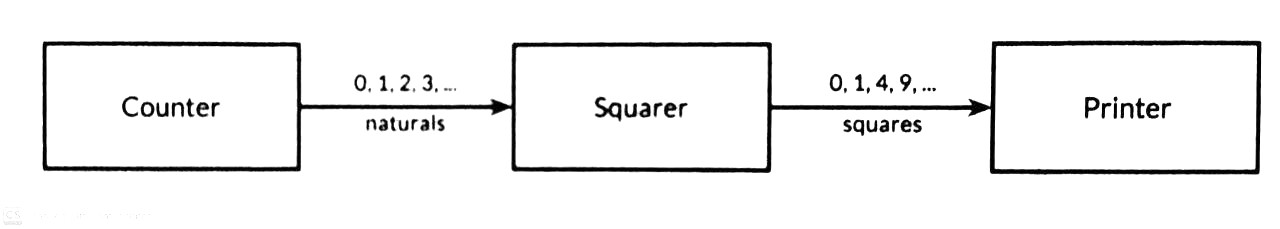
\includegraphics[width=0.8\linewidth]{figures/figure7.1}
\end{center}
La prima goroutine, \textit{counter}, genera gli interi 0, 1, 2, \ldots, e li invia su un channel alla seconda goroutine, \textit{squarer}, che riceve ogni valore, lo eleva al quadrato, e invia il risultato su un altro channel alla terza goroutine, \textit{printer}, che riceve i valori e li stampa.
Per chiarezza di quest'esempio, si è intenzionalmente scelto una funzione davvero semplice per spiegare il funzionamento della pipeline.
\begin{lstlisting}[frame=single, label={lst:lstlisting7-4-2.1}]
func main() {
    naturals := make(chan int)
    squares := make(chan int)

    // Counter
    go func() {
        for x := 0; ; x++ {
            naturals <- x
        }
    }()

    // Squarer
    go func() {
        for {
            x := <-naturals
            squares <- x * x
        }
    }()

    // Printer (nella main goroutine)
    for {
        fmt.Println(<-squares)
    }
}
\end{lstlisting}
Se il mittente conosce che non ci sono più valori da inviare sul channel, è bene comunicarlo alla goroutine destinataria così da non farlo attendere.
Questo è realizzato con la \textit{chiusura} del channel con la funzione built-in \verb|close|:
\begin{lstlisting}[frame=single, label={lst:lstlisting7-4-2.2}]
close(naturals)
\end{lstlisting}
Dopo che un channel è stato chiuso, qualunque altra operazione di send restituirà un panic.
Dopo che il channel chiuso sia stato \textit{svuotato}, ovvero dopo che l'ultimo elemento inviato sia stato recepito, tutte le successive operazioni di receive verranno risolte restituendo un valore zero per il tipo elementare del channel.
Chiudendo il channel \verb|naturals| si causerà al ciclo di squarer di ricevere uno stream senza fine di valori zero, e di inviare tali valori al printer.

Non esiste un modo diretto per capire se un channel è stato chiuso, ma esiste una variante dell'operazione di receive che produce due risultati: l'elemento ricevuto dal channel più un valore booleano, denominato per convenzione \verb|ok|, che è \verb|true| nel caso di un'operazione di receive completata con successo e \verb|false| nel caso di un'operazione di receive su un channel chiuso e svuotato.
Usando questa funzionalità, il ciclo di squarer può essere modificato così da interromperlo quando il channel \verb|naturals| è svuotato e chiudere a cascata il channel \verb|squares|.
\begin{lstlisting}[frame=single, label={lst:lstlisting7-4-2.3}]
go func() {
    for {
        x, ok := <-naturals
        if !ok {
            break // il channel %*\textit{è}*\) stato chiuso e svuotato
        }
        squares <- x * x
    }
    close(squares)
}()
\end{lstlisting}
Il linguaggio permette di usare un ciclo \verb|range| per iterare anche su un channel.
Questo è sintatticamente più conveniente per ricevere tutti i valori inviati su un channel e terminare il ciclo dopo l'ultimo.
\begin{lstlisting}[frame=single, label={lst:lstlisting7-4-2.4}]
func main() {
    naturals := make(chan int)
    squares := make(chan int)

    // Counter
    go func() {
        for x := 0; x < 100; x++ {
            naturals <- x
        }
        close(naturals)
    }()

    // Squarer
    go func() {
        for x := range naturals {
            squares <- x * x
        }
        close(squares)
    }()

    // Printer (nella main goroutine)
    for x := range squares {
        fmt.Println(x)
    }
}
\end{lstlisting}
Non è sempre necessario chiudere un channel, lo è nel momento in cui è importante avvisare la goroutine destinaria che tutti i valori sono stati inviati, altrimenti può anche essere tralasciato perché il garbage collector si occuperà di determinare quando un channel è diventato irraggiungibile e quindi riciclarlo anche se non chiuso.
(Questo discorso non vale per i file;
i file devono sempre essere chiusi tramite chiamata al metodo \verb|Close|).

\subsection{Tipi di channel unidirezionali}
\label{subsec:tipi_di_channel_unidirezionali}%
Non appena un programma cresce, è naturale spezzare grandi funzioni in pezzi più piccoli.
La funzione \verb|main| proposta alle pagine precedenti può essere suddivisa in tre funzioni:
\begin{lstlisting}[frame=single, label={lst:lstlisting7-4-3.1}]
func counter(out chan int)
func squarer(out, in chan int)
func printer(in chan int)
\end{lstlisting}
La funzione \verb|squarer|, posto in mezzo alla pipeline, riceve due parametri, il channel di input e il channel di output.
Entrambi hanno lo stesso tipo, ma i loro usi opposti: \verb|in| è solo per ricevere, mentre \verb|out| solo per inviare.
I nomi \verb|in| e \verb|out| rafforzano questa idea, ma nulla vieta a \verb|squarer| di inviare su \verb|in| e di ricevere da \verb|out|.

Quando un channel è passato come parametro di una funzione, è quasi sempre dato con l'intento di usarlo esclusivamente per inviare o esclusivamente per ricevere.

Per documentare questo intento e prevenire un uso scorretto, il type system di Go offre i tipi di channel \textit{unidirezionali} per permettere solo una fra le operazioni di send e receive.
Il tipo \verb|chan<- int|, un channel di \textit{solo invio} di \verb|int|, permette solo gli invii.
Al contrario, il tipo \verb|<-chan int|, un channel di \textit{sola ricezione} di \verb|int|, permette solo le ricezioni.
Violazioni di questi usi sono individuati a compile time.

Dato che l'operazione di \verb|close| asserisce che nessuna operazione di send verrà più effettuata su un channel, allora solo la goroutine mittente potrà chiamarla, e per questa ragione è un errore a compile time provare a chiudere un channel di sola ricezione.
\begin{lstlisting}[frame=single, label={lst:lstlisting7-4-3.2}]
func counter(out chan<- int) {
    for x := 0; x < 100; x++ {
        out <- x
    }
    close(out)
}

func squarer(out chan<- int, int <-chan int) {
    for v := range in {
        out <- v * v
    }
    close(out)
}

func printer(in <-chan int) {
    for v := range in {
        fmt.Println(v)
    }
}
\end{lstlisting}
\begin{lstlisting}[frame=single, label={lst:lstlisting7-4-3.3}]
func main() {
    naturals := make(chan int)
    squares := make(chan int)

    go counter(naturals)
    go squarer(squares, naturals)
    printer(squares)
}
\end{lstlisting}
La chiamata \verb|counter(naturals)| converte \verb|naturals| dal tipo \verb|chan int| al tipo \verb|chan<- int| in modo implicito.
La chiamata a \verb|printer(squares)| esegue implicitamente una conversione simile a \verb|<-chan int|.
Le conversioni dei tipi di channel da bidirezionali a unidirezionali sono permesse in ogni assegnazione.
Non esiste però modo di tornare indietro: un channel convertito in unidirezionale non può più tornare ad essere bidirezionale.

\subsection{Buffered channel}
\label{subsec:buffered_channel}%
Un buffered channel ha una coda di elementi.
La dimensione massima della coda è decisa quando viene creato il channel, dall'argomento capacity in \verb|make|.
La seguente istruzione crea un buffered channel in grado di ospitare al più tre valori \verb|string|.
La figura mostra anche una rappresentazione di \verb|ch| e del channel a cui si riferisce.
\begin{lstlisting}[frame=single, label={lst:lstlisting7-4-4.1}]
ch = make(chan string, 3)
\end{lstlisting}
\begin{center}
    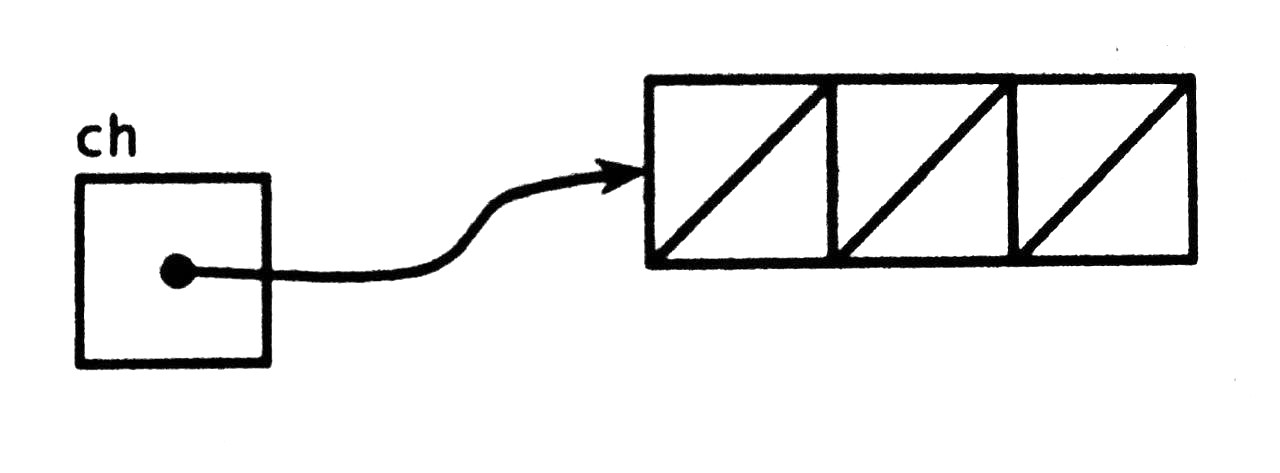
\includegraphics[width=0.5\linewidth]{figures/figure7.2}
\end{center}
Un'operazione di send su un buffered channel inserisce un elemento in coda alla fila d'attesa , e l'operazione di receive rimove un elemento dalla testa della fila.
Se il channel è pieno, l'operazione di send blocca la propria goroutine fino a quando non viene fatto spazio in seguito all'operazione di receive di un'altra goroutine.
Al contrario, se il channel è vuoto, un'operazione di receive blocca la propria goroutine fino a quando un'altra goroutine non esegue un'operazione di send sullo stesso channel.
\begin{lstlisting}[frame=single, label={lst:lstlisting7-4-4.2}]
ch <- %*``*\)A%*''*\)
ch <- %*``*\)B%*''*\)
ch <- %*``*\)C%*''*\)
\end{lstlisting}
Dopo aver eseguito queste tre istruzioni, il channel è pieno e una quarta operazione di send verrà bloccata.
\begin{center}
    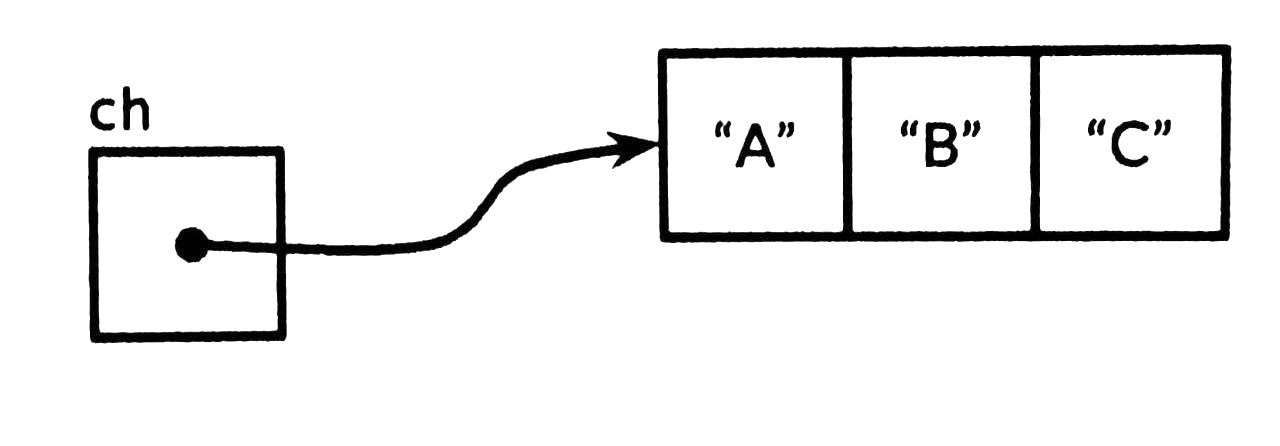
\includegraphics[width=0.5\linewidth]{figures/figure7.3}
\end{center}
Se si riceve un valore,
\begin{lstlisting}[frame=single, label={lst:lstlisting7-4-4.3}]
fmt.Println(<-ch)
\end{lstlisting}
Output:
\begin{lstlisting}[language=bash, frame=L, label={lst:lstlisting7-4-4.4}]
A
\end{lstlisting}
il channel non sarà più nè pieno nè vuoto, quindi sia un'operazione di send che una di receive potranno procedere senza essere bloccati.
In questo modo, il buffer del channel separa le goroutine mittenti e destinatari.
\begin{center}
    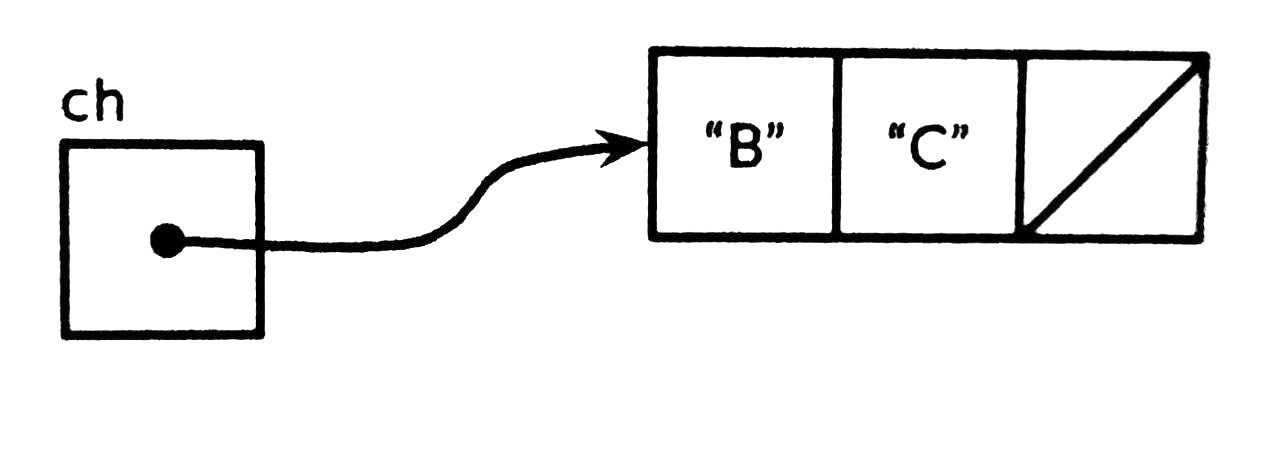
\includegraphics[width=0.5\linewidth]{figures/figure7.4}
\end{center}
Nel caso un programma voglia conoscere la capacità del buffer del channel può richiamare la funzione \verb|cap|:
\begin{lstlisting}[frame=single, label={lst:lstlisting7-4-4.5}]
fmt.Println(cap(ch))
\end{lstlisting}
Output:
\begin{lstlisting}[language=bash, frame=L, label={lst:lstlisting7-4-4.6}]
3
\end{lstlisting}
Quando applicato al channel, la funzione \verb|len| restituisce il numero di elementi al momento presenti nel buffer.

Il seguente esempio presenta un'applicazione di un buffered channel.
Tale programma fa richieste in parallelo a tre \textit{mirror}, ovvero server equivalenti ma geograficamente distribuiti.
Essi inviano la loro risposta su un buffered channel, quindi ricevono e restituiscono solo la prima risposta, che è la più veloce ad arrivare.
Quindi \verb|mirrorQuery| restituisce un risultato anche prima della risposta dei due server più lenti.
\begin{lstlisting}[frame=single, label={lst:lstlisting7-4-4.7}]
func mirrorQuery() string {
responses := make(chan string, 3)
    go func() { responses <- request(%*``*\)asia.gopl.io%*''*\)) }()
    go func() { responses <- request(%*``*\)europe.gopl.io%*''*\)) }()
    go func() { responses <- request(%*``*\)americas.gopl.io%*''*\)) }()
    return <-responses // Ritorna la risposta pi%*\textit{ù}*\) veloce
}

func request(hostname string) (response string) { /* ... */ }
\end{lstlisting}
La scelta fra un unbuffered e buffered channel e la scelta della capacity per il buffered channel possono entrambe influenzare la correttezza del programma.
Gli unbuffered channel offrono una forte garanzia di sincronizzazione perché ogni operazione di send è sincronizzata con la corrispettiva operazione di receive;
con i buffered channel, queste operazioni sono slegate.
Inoltre, quando si conosce la dimensione massima del numero di valori che possono essere inviati su un channel, è utile creare un buffered channel di quella dimensione ed effettuare tutti i send ancor prima che il primo valore sia ricevuto dal destinatario.
Un fallimento nell'allocazione di un buffer di sufficiente capacity potrebbe portare il programma ad un deadlock.

\section{Esempio: Chat Server}
\label{sec:esempio_chat_server}
%
Un chat server permette a molti utenti di inviarsi l'un l'altro messaggi testuali.
Ci sono quattro tipologie di goroutine in questo programma.
C'è un'istanza a testa per la goroutine \verb|main| e \verb|broadcast|, e per ogni connessione client c'è una goroutine \verb|handleConn| e una \verb|clientWriter|.

Il compito della main goroutine è rimanere in ascolto e di accettare connessioni di rete in input da parte di client.
Per ognuno di essi, il main crea una nuova goroutine \verb|handleConn|.
\begin{lstlisting}[frame=single, label={lst:lstlisting7-10.1}]
func main() {
    listener, err := net.Listen(%*``*\)tcp%*''*\), %*``*\)localhost:8000%*''*\))
    if err != nil {
        log.Fatal(err)
    }

    go broadcaster()
    for {
        conn, err := listener.Accept()
        if err != nil {
            log.Print(err)
            continue
        }
        go handleConn(conn)
    }
}
\end{lstlisting}
Il broadcaster ha una variabile locale \verb|clients| che tiene registrato l'insieme di tutti i client correntemente connessi.
Per ogni client viene memorizzata solo l'identità del loro channel di messaggi in uscita.
\begin{lstlisting}[frame=single, label={lst:lstlisting7-10.2}]
type client chan<- string // un channel di messaggi in uscita

var (
    entering = make(chan client)
    leaving  = make(chan client)
    messages = make(chan string) // tutti i messaggi client in
                                 // arrivo
)

func broadcaster() {
    clients := make(map[client]bool) // tutti i client connessi
    for {
        select {
        case msg := <-messages:
            // Trasmette il messaggio in entrata ai
            // channel dei messaggi in uscita di tutti i client.
            for cli := range clients {
                cli <- msg
            }
        case cli := <-entering:
            clients[cli] = true
        case cli := <-leaving:
            delete(clients, cli)
            close(cli)
        }
    }
}
\end{lstlisting}
Il broadcaster rimane in ascolto sui channel globali \verb|entering| e \verb|leaving| per annunci sull'arrivo o sulla partenza di client.
Quando riceve un annuncio di questi eventi, aggiorna l'insieme \verb|clients|, e se l'evento è di partenza, chiude il channel di messaggi in uscita del client corrispondente.
Il broadcaster rimane anche in ascolto di eventi sul channel globale \verb|messages|, dove ogni client invia tutti i suoi messaggi in arrivo.
Quando il broadcaster riceve uno di questi eventi, invia a tutti i client connessi il messaggio.

Ora si veda la goroutine dedicata al client sul server.
La funzione \verb|handleConn| crea un channel di messaggi in uscita per il proprio client e annuncia l'arrivo dello stesso client al broadcaster sul channel \verb|entering|.
A questo punto legge ogni linea di testo dal client, invia ogni linea al broadcaster sul channel di messaggi in arrivo, aggiungendo come prefisso ad ogni messaggio l'identità del mittente.
Una volta che non c'è più nulla da leggere dal client, \verb|handleConn| annuncia la partenza del client sul channel \verb|leaving| e chiude la connessione.
\begin{lstlisting}[frame=single, label={lst:lstlisting7-10.3}]
func handleConn(conn net.Conn) {
    ch := make(chan string) // messaggi client in uscita
    go clientWriter(conn, ch)

    who := conn.RemoteAddr().String()
    ch <- %*``*\)You are %*''*\) + who
    messages <- who + %*``*\) has arrived%*''*\)
    entering <- ch

    input := bufio.NewScanner(conn)
    for input.Scan() {
        messages <- who + %*``*\): %*''*\) + input.Text()
    }
    // NOTA: si ignorano potenziali errori di input.Err()

    leaving <- ch
    messages <- who + %*``*\) has left%*''*\)
    conn.Close()
}

func clientWriter(conn net.Conn, ch <-chan string) {
    for msg := range ch {
        fmt.Fprintln(conn, msg) // NOTA: si ignorano gli errori
                                // di rete
    }
}
\end{lstlisting}
In aggiunta, \verb|handleConn| crea una goroutine \verb|clientWriter| per ogni client che riceve un messaggio in broadcast sul channel di messaggi in uscita del client e li scrive sulla connessione di rete del client.
Il ciclo del writer del client termina quando il broadcaster chiude il channel dopo aver ricevuto la notifica di \verb|leaving|.

Per il lato client invece viene utilizzato il programma esposto nel paragrafo \textbf{Unbuffered channel} di questo capitolo.
Una simulazione da linea di comando:
\begin{lstlisting}[language=bash, frame=L, label={lst:lstlisting7-10.4}]
$ go build chat
$ go build netcat3
$ ./chat &
$ ./netcat3
You are 127.0.0.1:64208         $ ./netcat3
127.0.0.1:64211 has arrived     You are 127.0.0.1:64211
Hi!
127.0.0.1:64208: Hi!            127.0.0.1:64208: Hi!
                                Hi yourself.
127.0.0.1:64211 Hi yourself.    127.0.0.1:64211: Hi yourself.
^C
                                127.0.0.1:64208 has left
$ ./netcat3
You are 127.0.0.1:64216         127.0.0.1:64216 has arrived
                                Welcome.
127.0.0.1:64211: Welcome.       127.0.0.1:64211: Welcome.
                                ^C
127.0.0.1:64211 has left
\end{lstlisting}
Mentre il server ospita una sessione di chat per $n$ client, il programma esegue $2n+2$ goroutine comunicanti in modo concorrente, anche se necessita di un'esplicita operazione di lock.
La \verb|clients| map è confinata in una singola goroutine, nel broadcaster, così non può essere acceduta in modo concorrente.
Le uniche variabili condivise fra più goroutine sono i channel e le istanze di \verb|net.Conn|, i quali sono entrambi \textit{concurrency safe}.

